\documentclass[UTF8]{article} 
\usepackage{graphicx}
\usepackage{subfigure}
\usepackage{amsmath}
\usepackage{makecell}
\usepackage[utf8]{inputenc}
\usepackage[space]{ctex} %中文包
\usepackage{listings} %放代码
\usepackage{xcolor} %代码着色宏包
\usepackage{CJK} %显示中文宏包
\usepackage{float}


\definecolor{mygreen}{rgb}{0,0.6,0}
\definecolor{mygray}{rgb}{0.5,0.5,0.5}
\definecolor{mymauve}{rgb}{0.58,0,0.82}
\lstset{
	backgroundcolor=\color{white}, 
	basicstyle = \footnotesize,       
	breakatwhitespace = false,        
	breaklines = true,                 
	captionpos = b,                    
	commentstyle = \color{mygreen}\bfseries,
	extendedchars = false,             
	frame =shadowbox, 
	framerule=0.5pt,
	keepspaces=true,
	keywordstyle=\color{blue}\bfseries, % keyword style
	language = Verilog,                     % the language of code
	otherkeywords={string}, 
	numbers=left, 
	numbersep=5pt,
	numberstyle=\tiny\color{mygray},
	rulecolor=\color{black},         
	showspaces=false,  
	showstringspaces=false, 
	showtabs=false,    
	stepnumber=1,         
	stringstyle=\color{mymauve},        % string literal style
	tabsize=4,          
	title=\lstname                      
}


\title{中国科学技术大学计算机学院\\《数字电路实验》报告}
\author{}

\date{}

\begin{document}
	\maketitle
	\begin{figure}[H]
		\centering
		
\includegraphics[width=2.5in]{xiaohui.jpg}\vspace{0.5cm}\\
		\large{
			实验题目:FPGA 原理及 Vivado 综合\\
			学生姓名:王章瀚\\
			学生学号:PB18111697\\
			完成日期:\today\\
		}\vspace{2cm}
		
		\large{计算机实验教学中心制\\2019年09月\\}
		\thispagestyle{empty}
		\clearpage  % 清除当页页码
	\end{figure}


	\section{实验目的}
	了解 ROM 工作原理\par
	了解 FPGA 工作原理\par
	学会使用 Vivado 工具进行综合\par
	
	\section{实验环境}
	PC 一台\par
	Windows 或 Linux 操作系统\par
	Logisim\par
	Vivado 工具\par
	Nexys4DDR 开发板或 FPGAOL 实验平台\par
	vlab.ustc.edu.cn\par
	
	\section{实验过程}
	\subsection{初识 FPGA}
	FPGA 是一种可编程逻辑器件。从功能上来说,可编程逻辑芯片与其它芯片有着本质的不同。这些芯片的电路结构都是确定的,无法进行更改,虽然有些芯片也支持编程,但都是在软件层面上完成的,不支持对电路结构的编程。可编程逻辑器件则不然,这类器件支持在电路层次进行编程。\par
	FPGA 是目前最主流的可编程逻辑芯片,除此之外还有 CPLD、PAL、GAL 等。\par
	
	\subsection{FPGA 基本结构}
	FPGA 内部包含了大量的可编程逻辑单元( CLB,Configurable Logic Blocks),通过可编程的交叉互连矩阵(SwitchMatrix)连接在一起。\par
	每个 CLB 内部包含两个 Slice, Slice 是 Xilinx 公司 FPGA 的最小单元。\par
	每个 Slice 都是由查找表( LUT, Look-Up Table)和触发器(FF,Flip-Flop)构成。查找表本质上来说就是一个 1bit 位宽的静态随机存储器(SRAM)。通过向 SRAM 加载编程数据,便能实现各种逻辑功能,可编程的互连资源能够将 CLB 级联起来,实现更为复杂的逻辑功能。\par
	\begin{figure}[H]
		\centering
		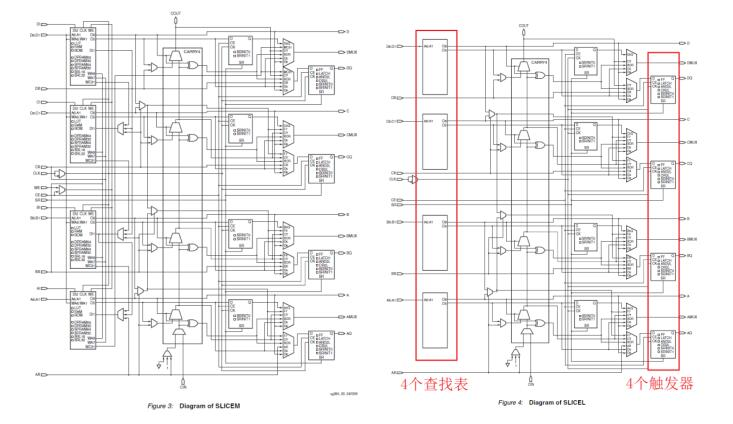
\includegraphics[width=1\linewidth]{s2.jpg}
		\label{s2}
	\end{figure}

	\subsection{可编程逻辑单元}
	以下是Slice结构的简化模型讲解。\par
	在Logisim中用RAM可以搭出下面电路:\par
	\begin{figure}[H]
		\centering
		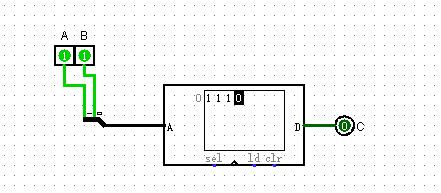
\includegraphics[width=1\linewidth]{s3_1.jpg}
		\label{s3_1}
	\end{figure}
	容易看出来,对于不同的存储,不同的输入都对应着一个输出。因此,完全可以用这样的电路搭建任何逻辑电路。比如上面这个电路,实际上就是个与非门电路,即$\overline{AB}$\par
	在 RAM 的输出后面添加一个触发器和选择器,并添加一个时钟信号,如下图所示,便实现了对组合逻辑和时序逻辑的支持,通过选择器选择输出信号是否被寄存。如下图:\par
	
	通过配置 RAM 的内容和选择器的选择信号, 以下两种语法格式的电路都可以支持:\par
	\begin{lstlisting}[language=Verilog]
	//1) 组合逻辑
	assign o = fun(a,b); 
	//2) 时序逻辑
	always@(posedge clk)
		o <= fun(a,b);
	\end{lstlisting}\par
	\begin{figure}[H]
		\centering
		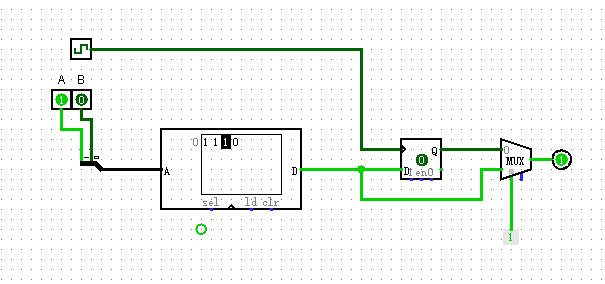
\includegraphics[width=1\linewidth]{s3_2.jpg}
		\label{s3_2}
	\end{figure}
	查找表和触发器共同构成了可编程逻辑单元。是 FPGA 中最核心最基本的单元。\par

	\subsection{交叉互连矩阵}
	当输入变量个数超出 LUT 输入数,或者需要进行信号反馈时,单靠可编程逻辑单元无法实现,这时候需要借助交叉互连矩阵的功能。以下为简化模型。\par
	在如下电路图中,通过修改选择器的选择信号,可以将任一输入信号输出到任意输出端口上去,也可以不输出到任何端口。\par
	\begin{figure}[H]
		\centering
		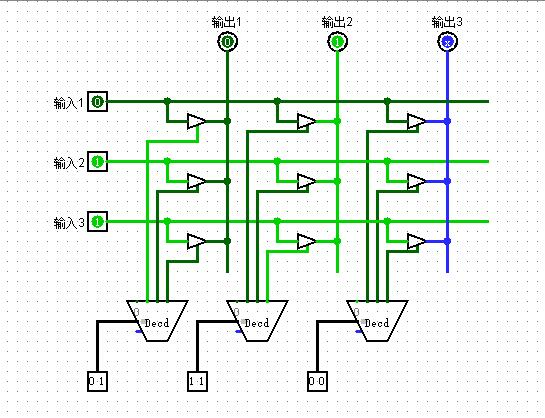
\includegraphics[width=1\linewidth]{s4.jpg}
		\label{s4}
	\end{figure}
	将可编程逻辑单元与交叉互连矩阵相连接,便能够实现信号的可编程逻辑单元的功能扩展和信号反馈。\par
	\begin{figure}[H]
		\centering
		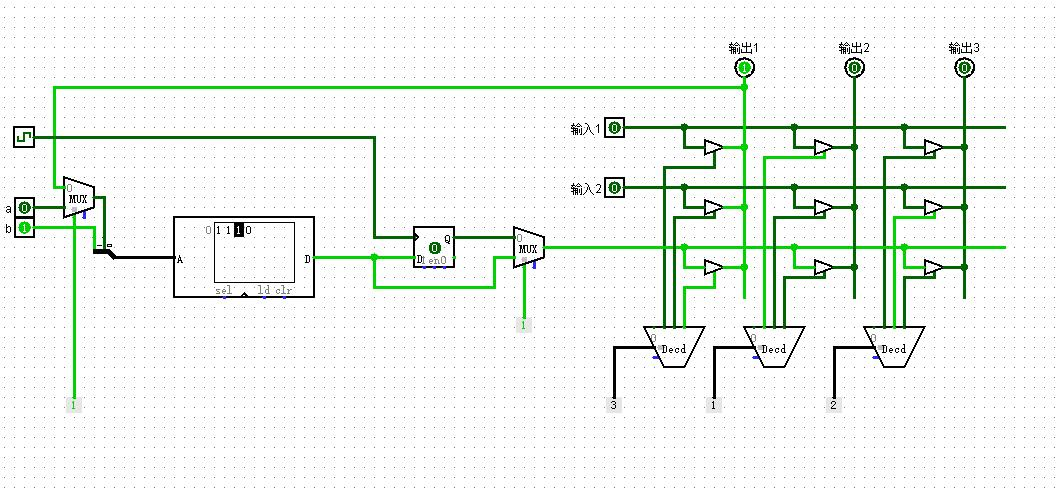
\includegraphics[width=1\linewidth]{s4_2.jpg}
		\label{s4_2}
	\end{figure}
	该电路能够支持如下格式的电路:\par
	\begin{lstlisting}[language=Verilog]
	//1) 更多变量的组合逻辑
	assign o = fun(a,b,输入 1,输入 2); 
	//2) 带反馈信号的时序逻辑
	always@(posedge clk) 
		a = fun(a,b);
	\end{lstlisting}\par
	所以,只要有足够的可编程逻辑单元和交叉互连矩阵资源,便可以实现所有逻辑电路。而用户需要做的事情就是在上图中配置区域内填入合适的数值。在Vivado中,这就是综合的过程。\par
	此外,FPGA 芯片的每一个通用管脚内部都有一个称为 IOB(Input/Output Block) 的控制模块,该模块可以控制管脚的输入输出状态,连接到交叉互连矩阵上,便能够实现将任意模块端口分配到该管脚的功能\par
	\begin{figure}[H]
		\centering
		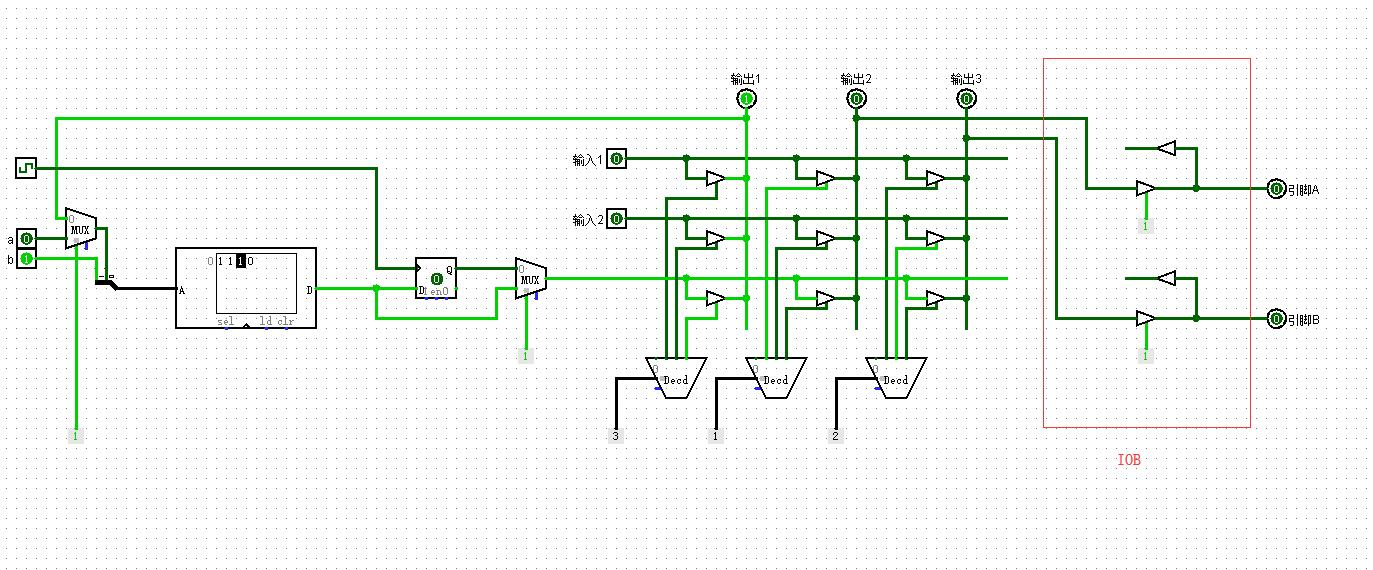
\includegraphics[width=1\linewidth]{s4_3.jpg}
		\label{s4_3}
	\end{figure}
	而IOB的信息,由xdc约束文件给出。这是专门用于引脚分配的文件。\par
	
	\subsection{Vivado 综合}
	按照教程编写代码。其管脚约束文件语法十分简单,如下:\par
	\begin{figure}[H]
		\centering
		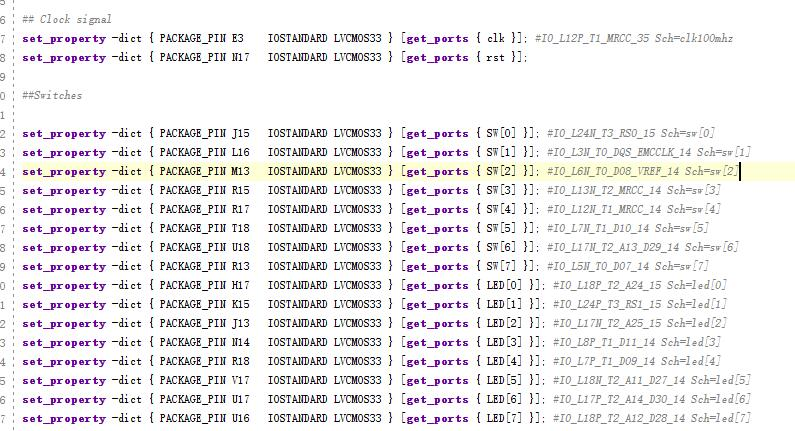
\includegraphics[width=1\linewidth]{s5_1.jpg}
		\label{s5_1}
	\end{figure}
	管脚约束文件的语法非常简单,“PACKAGE\_PIN” 后面跟的是 FPGA 芯片的管脚编号,“get\_ports” 后面跟的是 Verilog 设计文件顶层模块的端口信号。\par
	最后Generate Bitstream, 得到bit文件。
	\begin{figure}[H]
		\centering
		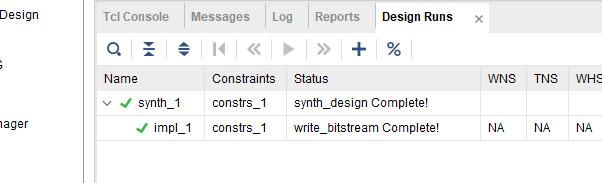
\includegraphics[width=1\linewidth]{s5_2.jpg}
		\label{s5_2}
	\end{figure}
	
	\subsection{烧写开发板}
	生成bit文件后,需要将其烧写到FPGA内。通过microUSB线缆将 Nexys4DDR 开发板和 PC 连接起来,识别设备后,写入。拨动开关,或按键,可以看到一些电路行为:\par
	\begin{figure}[H]
		\centering
		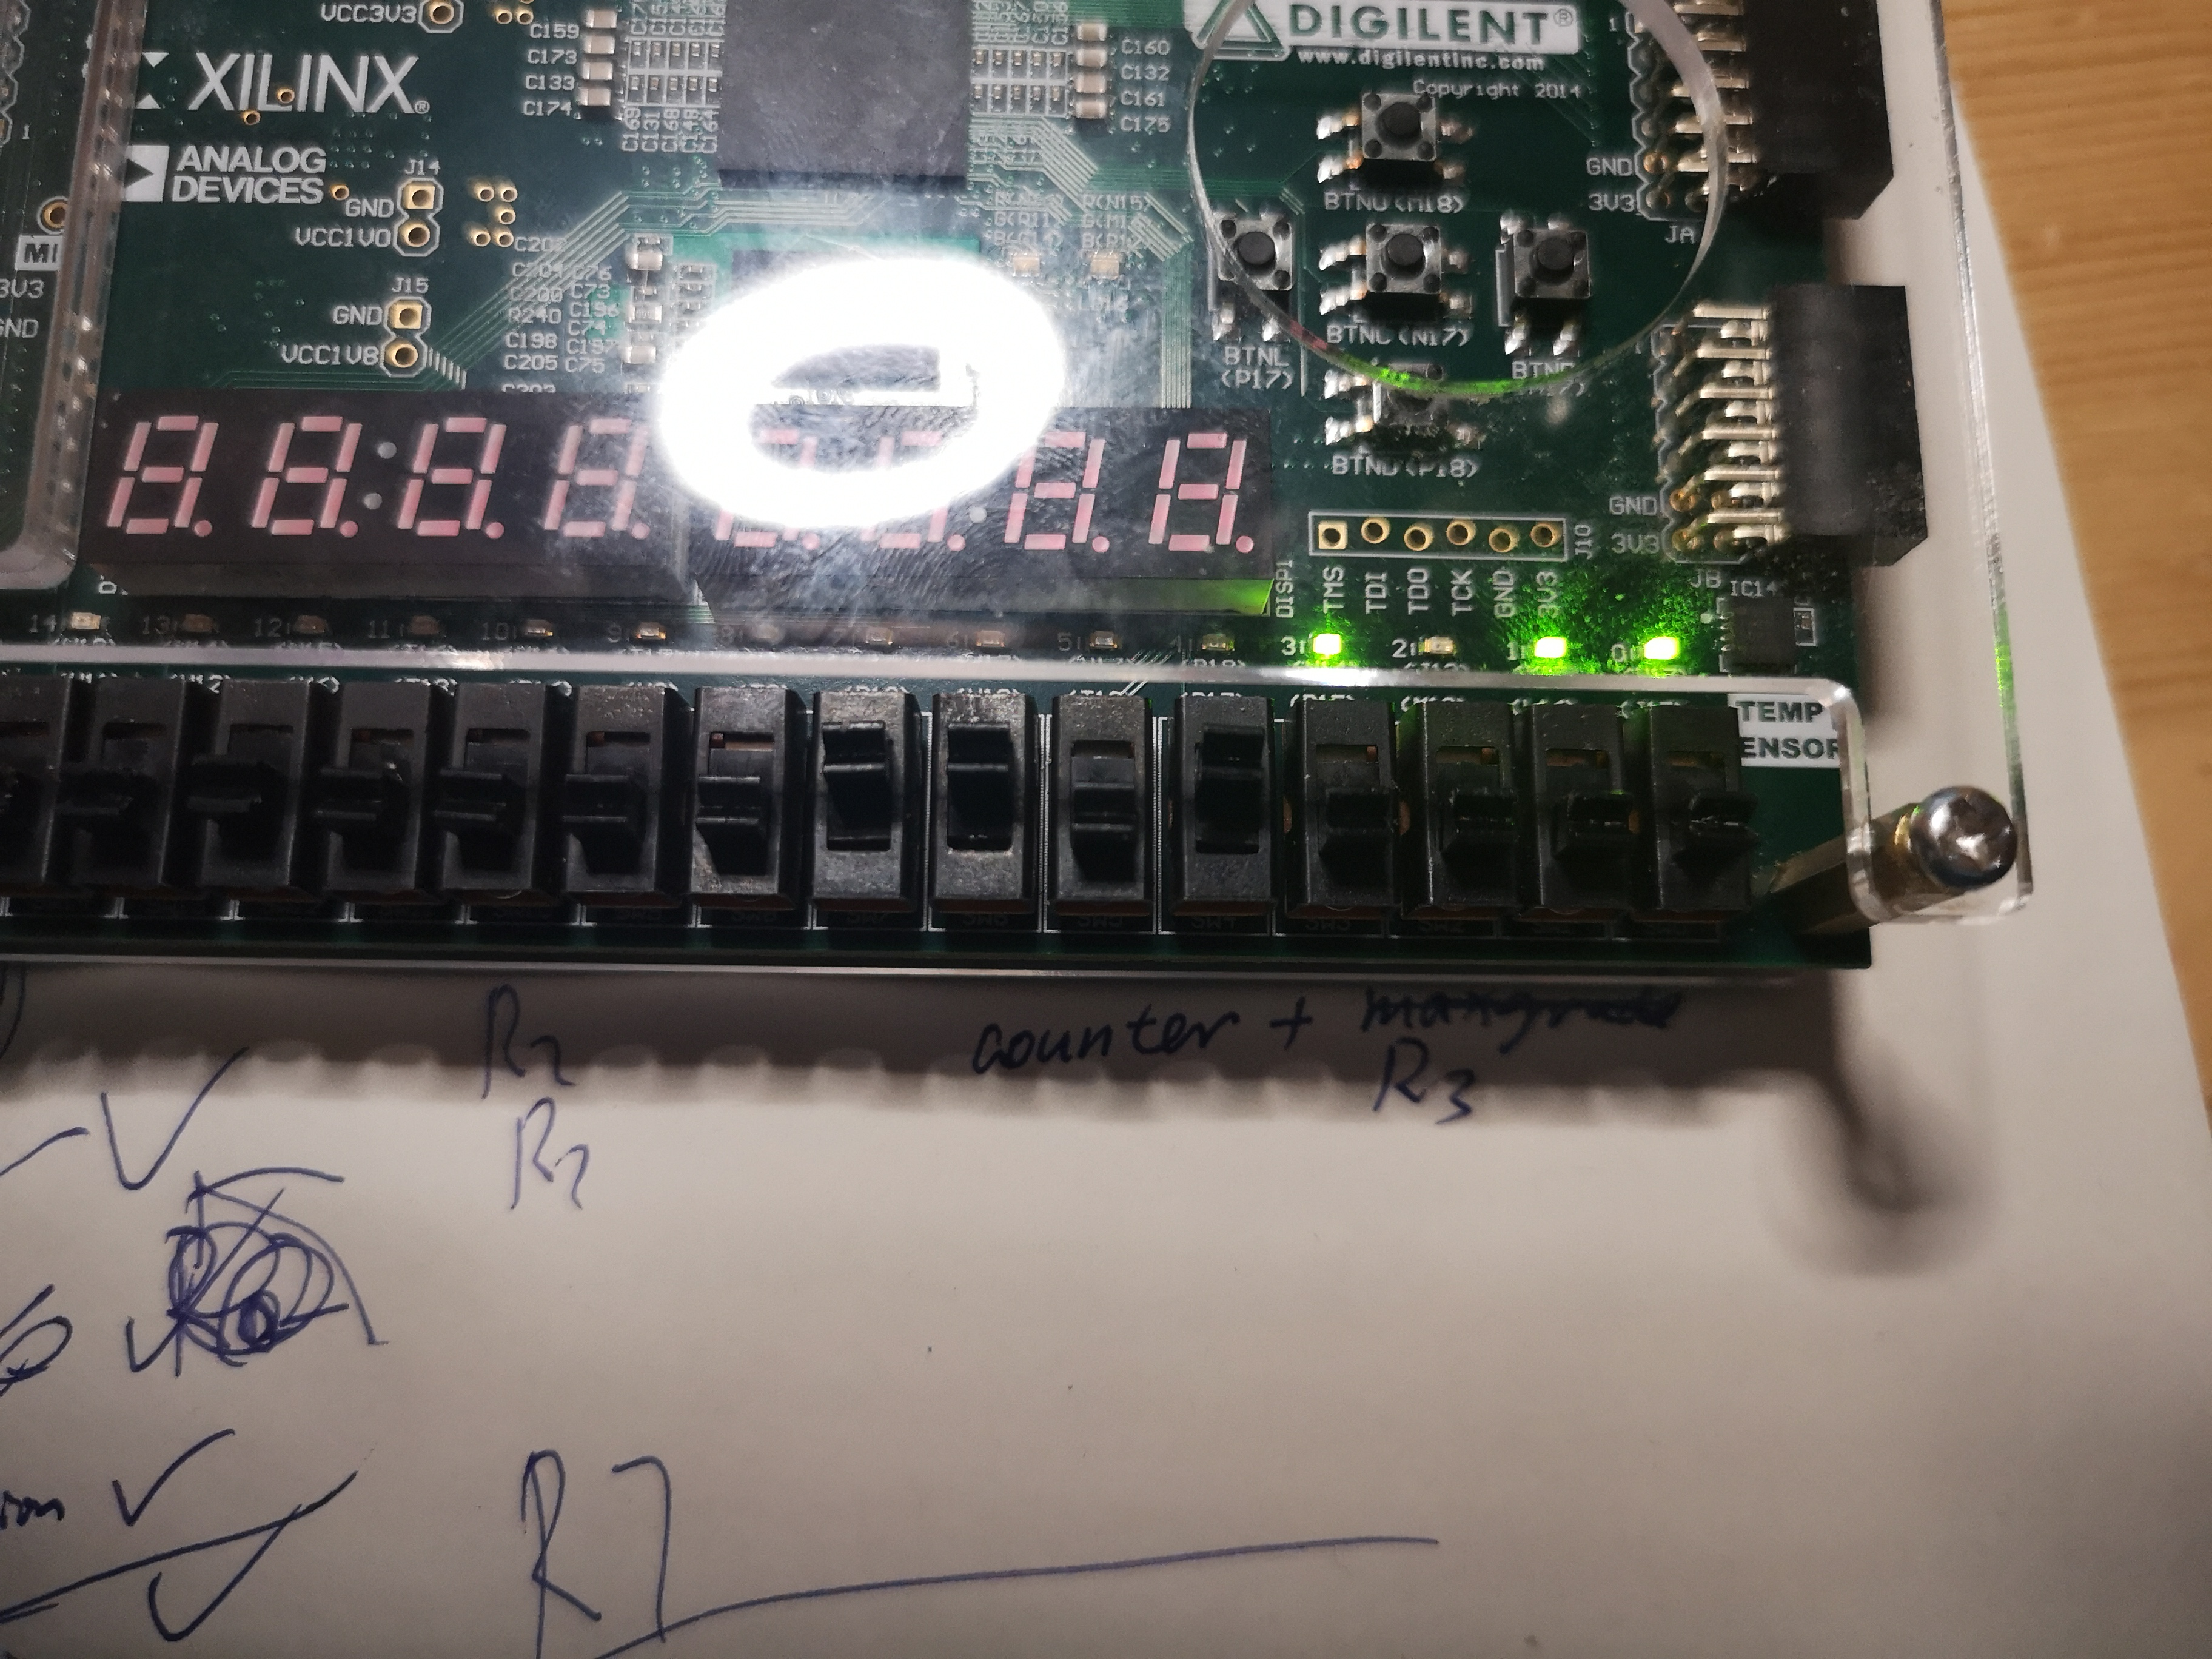
\includegraphics[width=1\linewidth]{s6.jpg}
		\label{s6}
	\end{figure}\par
	可以观察到,它确实实现了当开关i使能时,LED[7-i]亮灯。且rst可以做到异步复位。
	
	\section{实验练习}	
	\subsection{题目1}
	电路图设计如下:
	\begin{figure}[H]
		\centering
		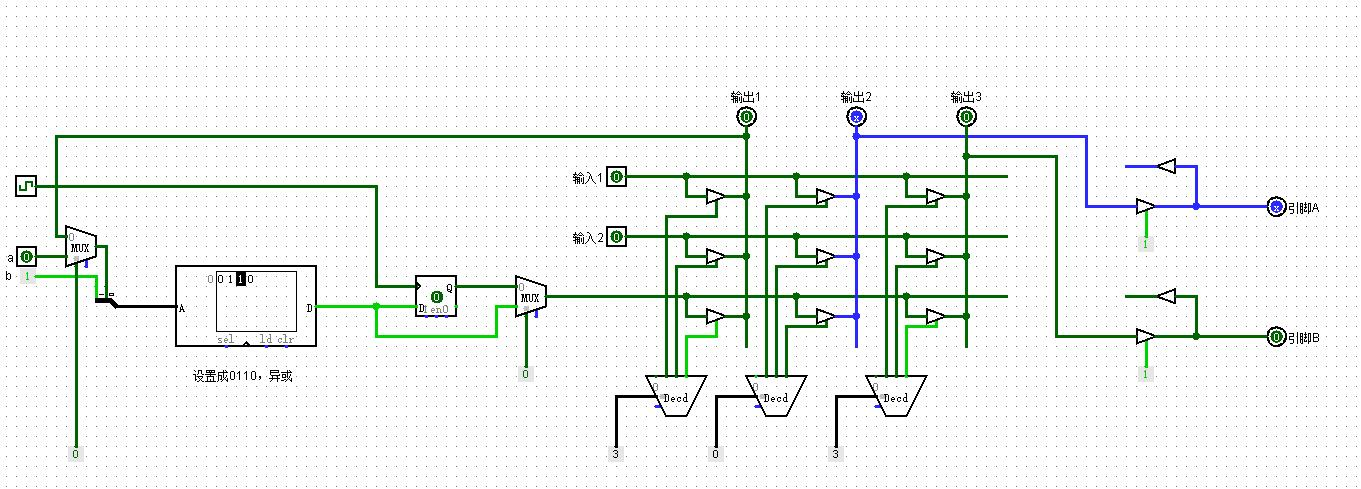
\includegraphics[width=1\linewidth]{e1.jpg}
		\label{e1}
	\end{figure}

	\subsection{题目2}
	只需修改约束文件如下:
	\begin{figure}[H]
		\centering
		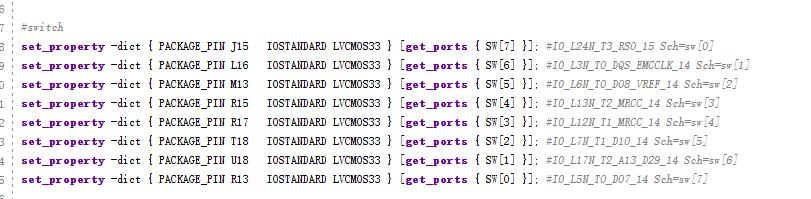
\includegraphics[width=1\linewidth]{e2.jpg}
		\caption{修改后约束文件}
		\label{e2}
	\end{figure}\par

	\begin{figure}[H]
		\centering
		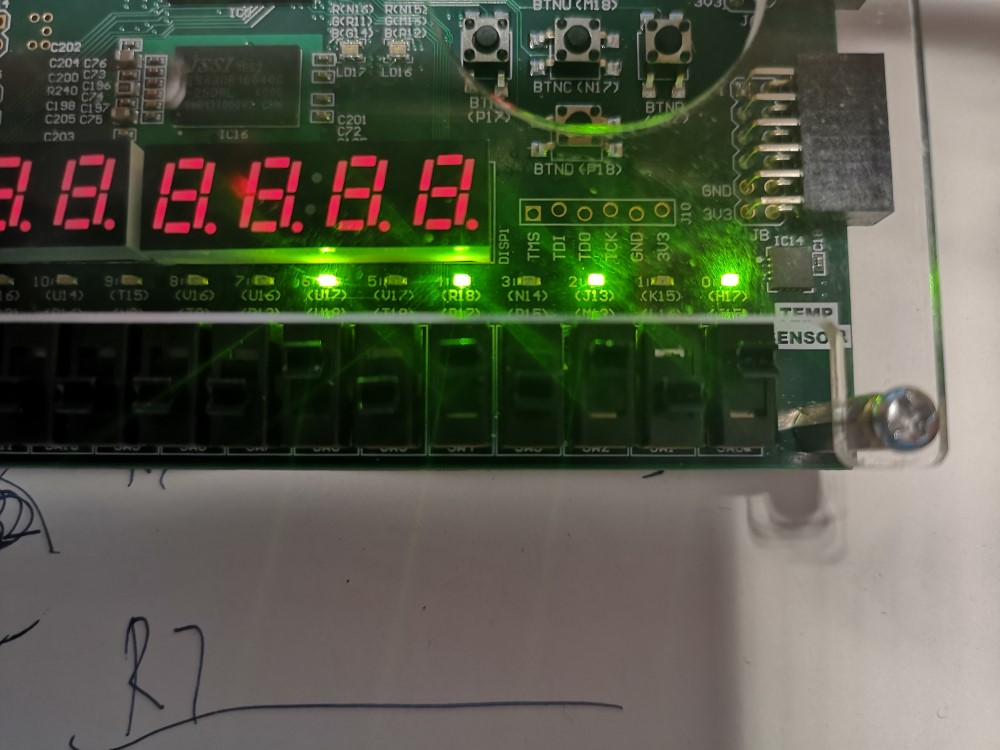
\includegraphics[width=1\linewidth]{e2_1.jpg}
		\caption{不按复位开关}
		\label{e2_1}
	\end{figure}\par
	\begin{figure}[H]
	\centering
	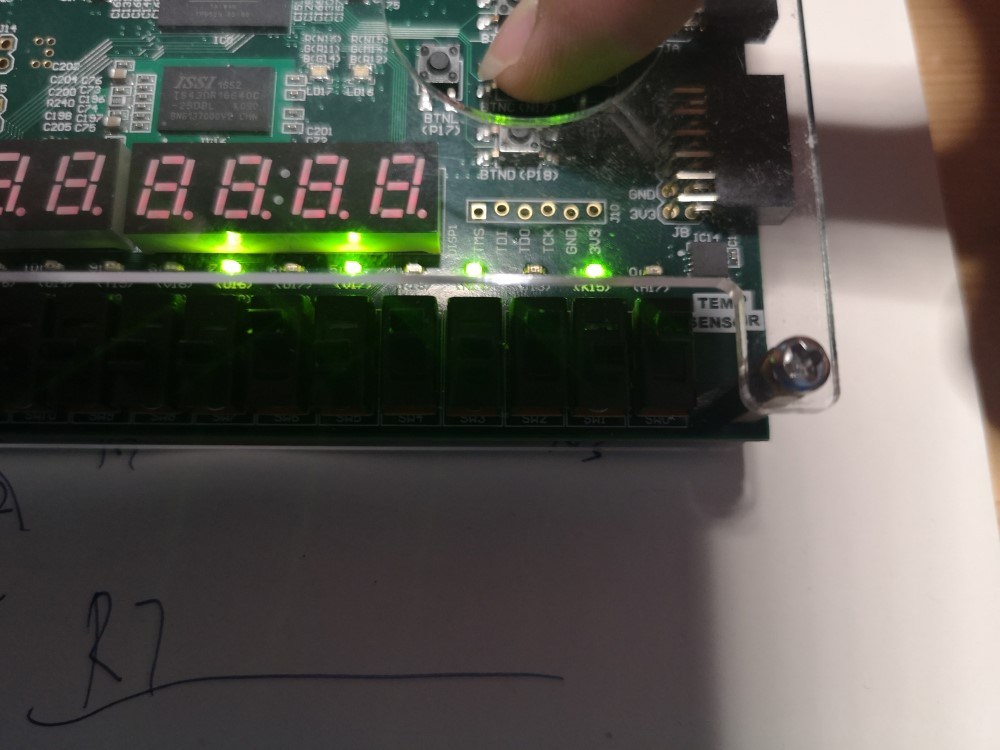
\includegraphics[width=1\linewidth]{e2_2.jpg}
	\caption{按下复位开关}
	\label{e2_2}
	\end{figure}\par
	
	
	\subsection{题目3}
	\subsubsection{8位计数器}
	程序如下:\par
	\begin{lstlisting}[language=Verilog]
	module e3_8bit(
		input clk,
		output reg [7:0] LED
		);
	
	initial
	begin
		LED = 8'b0000_0000;
	end
	
	always @(posedge clk)
	begin
		LED <= LED + 1;
	end
	
	endmodule
	\end{lstlisting}
	烧写后,效果如下图:\par
	\begin{figure}[H]
		\centering
		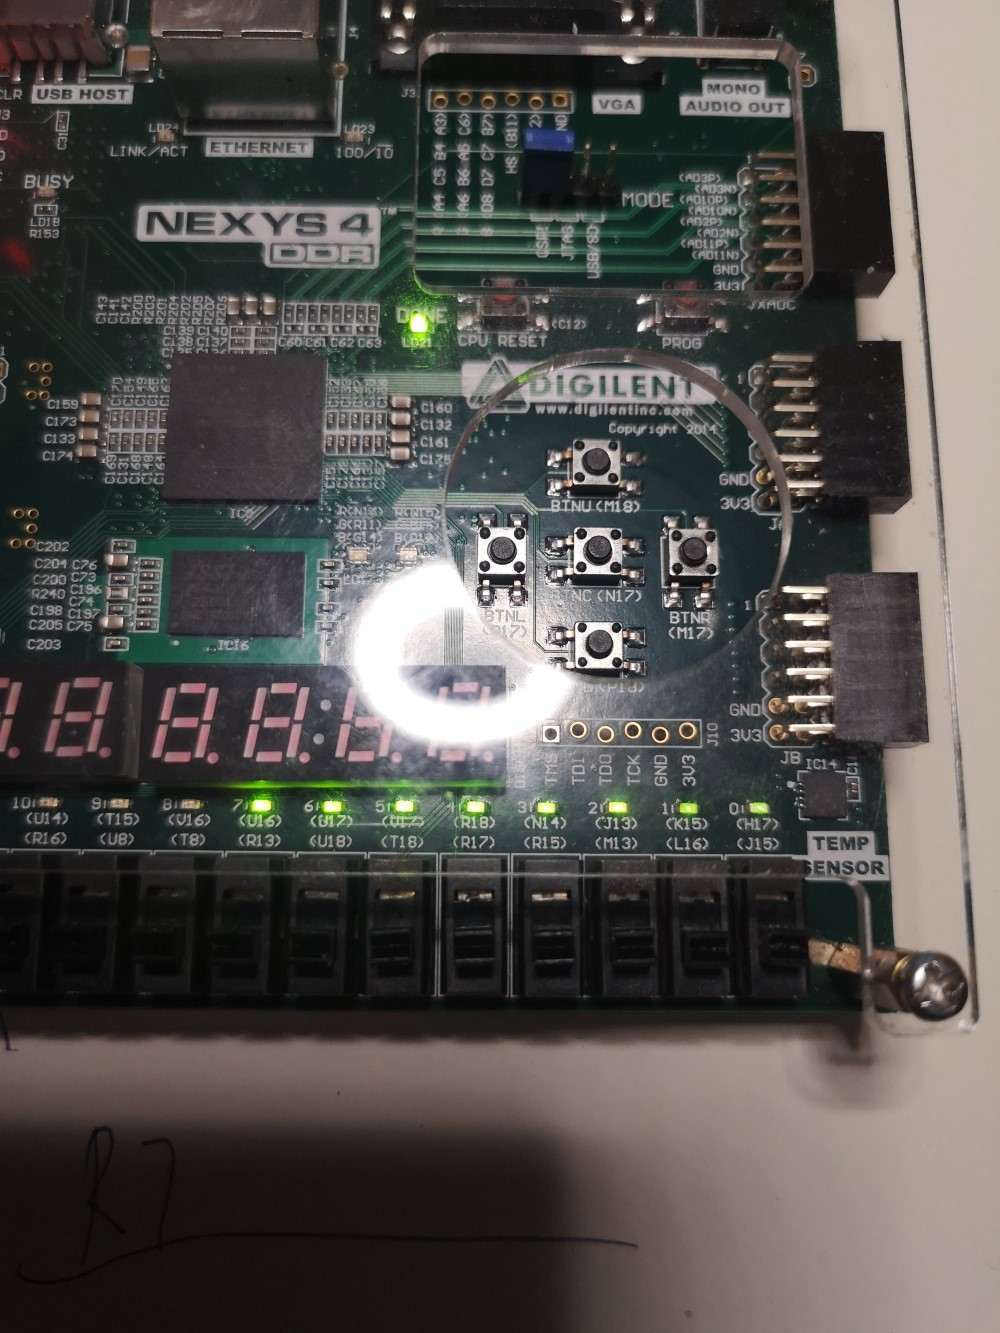
\includegraphics[width=0.5\linewidth]{e3_1.jpg}
		\caption{用8位计数器}
		\label{e3_1}
	\end{figure}\par
	造成这种效果的原因,我推测是时钟频率过高,导致看起来每个LED都是一直亮着的。\par
	
	\subsubsection{32位计数器}
	程序如下:\par
	\begin{lstlisting}[language=Verilog]
	module e3_8bit(
	input clk,
	output reg [7:0] LED
	);
	
	initial
	begin
	LED = 8'b0000_0000;
	end
	
	always @(posedge clk)
	begin
	LED <= LED + 1;
	end
	
	endmodule
	\end{lstlisting}
	烧写后,效果如下图:\par
	\begin{figure}[H]
		\centering
		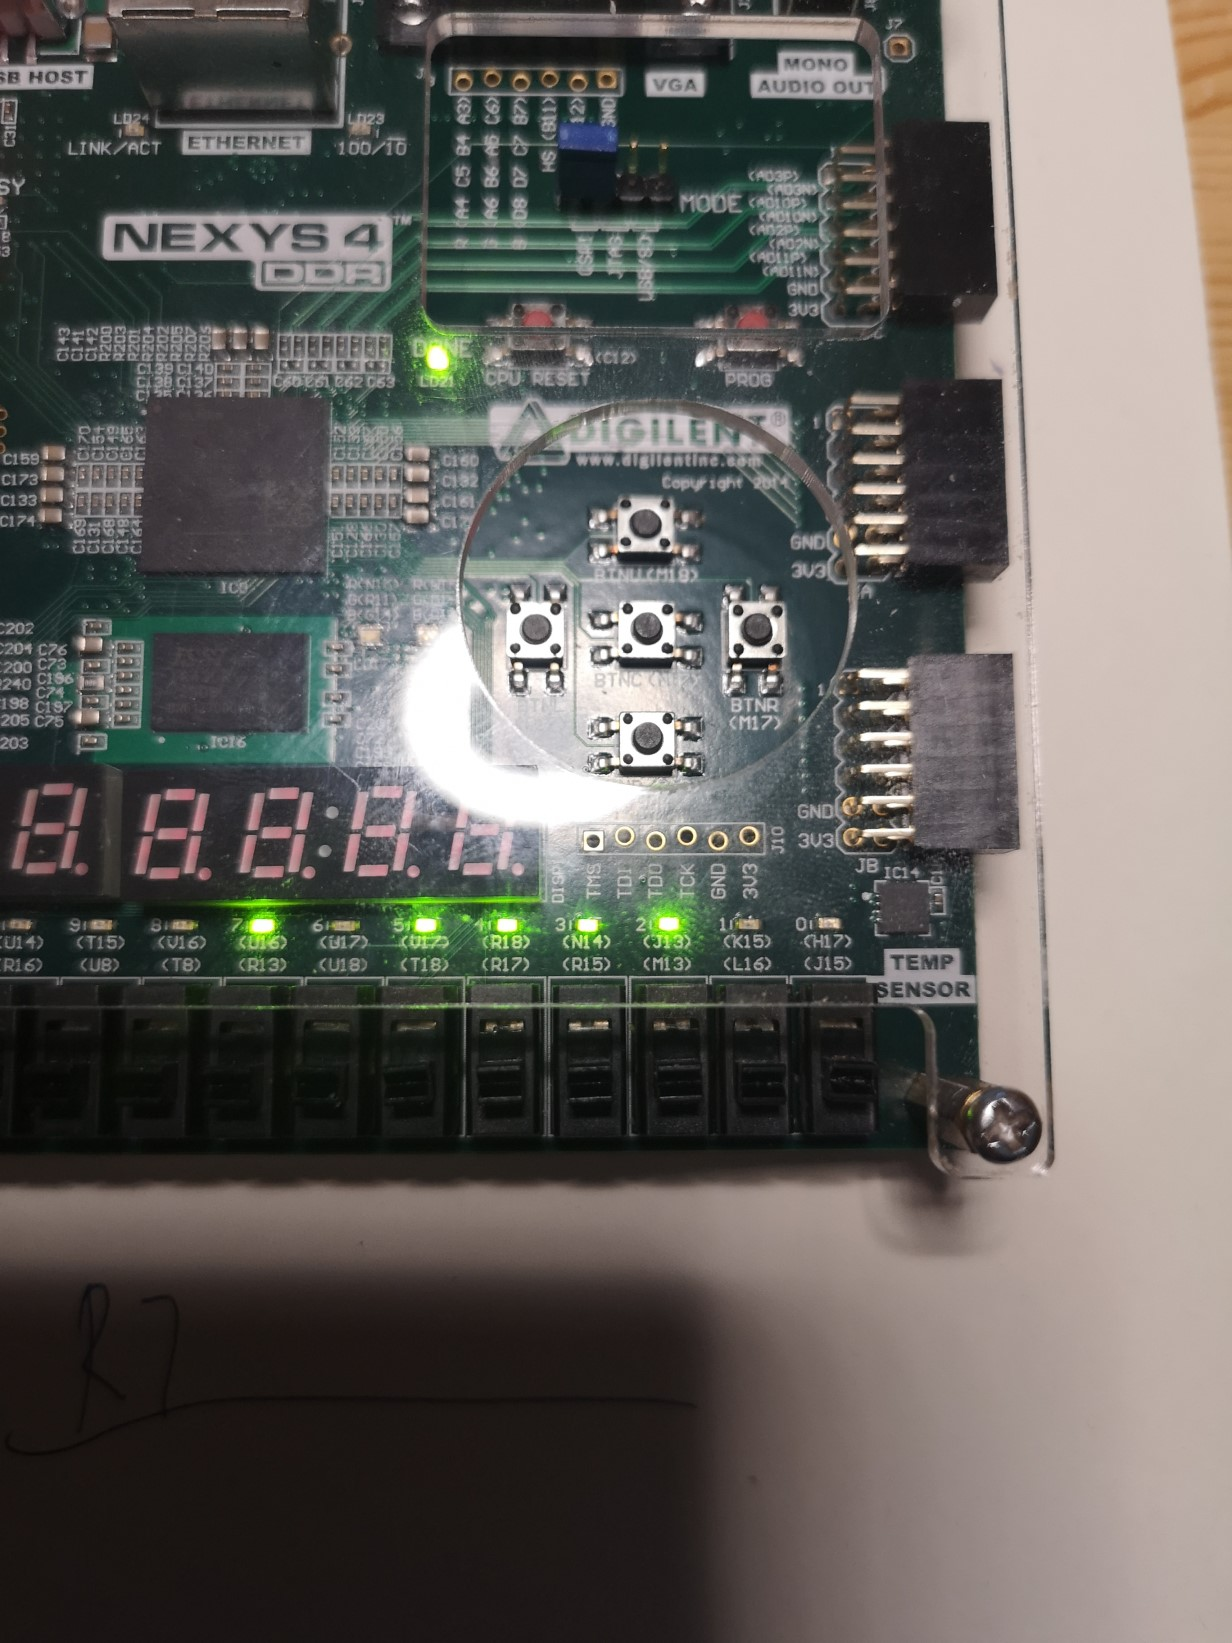
\includegraphics[width=0.5\linewidth]{e3_2.jpg}
		\caption{取32位计数器的高8位}
		\label{e3_2}
	\end{figure}\par
	由于取32位计数器的高8位,虽然时钟周期不变,但LED显示的周期变大了,此时整个LED的效果变得清晰可辨。\par
	
	\subsubsection{分析}
	由于时钟频率高,因此只有8位的计数器,每完成一个周期所用的时间很短,因此平均效果下,每个LED都是常亮的,只不过亮度没有最亮时那样。但用32位计数器,则周期变长,LED的反应跟得上电平的变化,此时就有清晰明确的计数效果。\par
	
	
	\section{总结与思考}	
	\subsection{本次实验的收获}
	在本次实验中,收获较大,学会了使用Vivado的综合与下载到FPGA上的方法。\par
	
	\subsection{评价本次实验的难易程度}
	本次实验内容难度适中。\par
	
	\subsection{评价本次实验的任务量}
	本次实验任务量合理。\par
	
	\subsection{为本次实验提供改进建议}
	建议详述语法方面的问题。
	
\end{document}
